\chapter{Vehicle Operating Cost Impacts}
\section{Introduction}
Vehicle costs are direct expenses that comprise the costs of vehicle ownership (fixed) and vehicle operation (variable). The latter category, typically referred to as vehicle operating costs (VOCs), varies with vehicle use and is typically expressed in cents per mile traveled by a vehicle. For most transportation modes, VOC involves energy use, tires, maintenance, repairs, and mileage-dependent depreciation. Fixed vehicle costs are those that are largely independent of vehicle use and are generally unaffected by transportation improvements; examples are insurance costs, time-dependent depreciation, financing, and storage. Such costs are therefore typically excluded from VOC impact evaluation of projects.\\\\
VOC savings or benefits of a transportation improvement or intervention simply refer to the reduction in vehicle operating costs compared to an existing situation or a base-case alternative.\\\\
For areawide or corridor-level projects involving multimodal systems, an improvement in any part of the system can affect VOCs of the other parts or other modes. For example, service improvement in commuter rail or provision of a bus rapid transit along a corridor can affect the level of service on highway facilities in the same corridor because the shift of some travelers from automobile to transit would lead to improved highway level of service due to reduced congestion and thus, lower vehicle operating costs at the highway section.\\\\
In this chapter we identify VOC components and factors and present a procedural framework for assessing the
VOC impacts of transportation improvements.
%%
\section{Components of Vehicle Operating Cost}
The components of vehicle operating cost are the individual items associated with vehicle operation on which expenses are directly incurred. These include the costs of energy needed to propel the vehicle, fluids, and other light consumables associated with mechanical working of the drivetrain, occasional replacement of the vehicle’s contact surfaces with the guideway, vehicle repair and maintenance, and vehicle depreciation.
\subsection{Fuel}
Fuel is a key component of vehicle operating costs. For highway vehicles for instance, fuel costs can account for 50 to 75\% of usage-related costs. Fuel cost can be estimated on the basis of fuel efficiency and unit fuel price. Fuel efficiency, in turn, depends primarily on vehicle class, type, age, and speed. Automobile associations, petroleum institutes, and government energy agencies publish fuel prices (dollars per gallon) on a regular basis. In the United States, the average prices of gasoline and diesel in 2005 were \$2.2 and \$2.4, respectively (USDOE, 2005b). Fuel prices for VOC computation purposes should be derived by subtracting the federal and state gasoline taxes from retail prices. On a mileage basis, the unit costs of fuel (including oil) in 2003–2004 ranged from approximately 7 cents per vehicle-mile for small autos to over 21 cents per vehicle-mile for large trucks (Barnes and Langworthy, 2003; AAA, 2005). Generally, very low speeds, steep uphill grades, and curves lead to higher fuel consumption rates and hence higher overall fuel costs. In the Highway Economic Requirements System (HERS) model (FHWA, 2002), the change in vehicle fuel efficiencies across the years is accounted for in VOC estimation using an adjustment factor.
%%
\subsection{Shipping Inventory}
The inventory cost of cargo (freight transportation) is a special category of user cost. The entity that ships the cargo (the client) is a user of a shipping service made available by a carrier. In the course of transporting perishable or valuable cargo, the client incurs holding costs that represent an opportunity cost: If at the beginning of the shipment, the client had a cash amount worth the cargo being shipped, such an amount would have earned some interest by the time the cargo reaches its destination. So by having the cargo transported, the client is foregoing some benefits. Higher inventory costs are generally directly related to cargo value, greater cargo perishability, higher prevailing opportunity cost of money, and slower speed of the shipping vehicle. To compute the inventory cost for a given vehicle class, an hourly discount rate is typically determined and multiplied by the average value of shipments undertaken by that vehicle class (FHWA, 2002). AASHTO (2003) recommends that the inventory costs of cargo per vehicle-mile should be applied to the unit user cost attributed to cargo-carrying transportation vehicles. The most significant VOC factors that affect the shipping inventory costs are speed and delay, but cargo value and interest rate also can be influential. Higher cargo value and interest rates and greater travel or transfer delay translate to higher unit costs of shipping inventory, and higher speeds lead to lower inventory costs. For example, at a 10\% interest rate, two trucks each shipping \$100,000 cargo, one traveling at 60 mph and the other at 50 mph, incur inventory costs of approximately 2.5 and 6 cents per mile, respectively (AASHTO, 2003).
%%
\subsection{Lubricating Oils for Mechanical Working of the Drivetrain}
The lubricating oil cost includes the cost of engine oil, transmission fluids, brake fluids, and other similar consumables associated with the operation of vehicle engine and drive train. Oil cost is a product of unit price (dollars/quart) and consumption rates (quarts/mile). The consumption rates depend on the amount of use as well as characteristics of the guideway and vehicle, and operational conditions such as speed, delay, grade, and curves. Typically, the cost of this set of VOC components is reported together with fuel costs, but some sources report them separately.
%%
\subsection{Preservation of the Vehicle-Guideway Contact Surface}
At their points of contact, both the vehicle and guideway experience deterioration due to wear and tear. For highways and runways, the vehicle contact is a tire; for railways, the contact is typically a steel wheel. Updated tire costs (2005 dollars) from the HERS technical report, are as follows: \$54.71 per tire for small autos, \$86.54 for medium-sized to large autos, \$95.39 for four-tire single-unit trucks, \$95.38 for sixtire single-unit trucks, \$230.10 for single-unit trucks of three or more axles, and \$569.74 for combination trucks. Of the various VOC factors, pavement condition, grade, curvature, and speed changes are those that most influence the rate of wear of contact surfaces.
%%
\subsection{Vehicle Repair and Maintenance}
Repair and maintenance costs are incurred on vehicle parts that need replacement or replenishment after some amount of use. For gasoline-powered vehicles, these include the cost of batteries, alternators, fuel pumps, air pump, tire rims, electrical parts such as bulbs and fuses, and so on. These costs also include costs of replacing parts due to crashes, misuse, or other adversarial factors. In some methodologies, the cost of vehicle repair and maintenance is not reported separately but is added to other nonfuel costs. In Year 2005 dollars, the unit cost of vehicle repair and maintenance generally ranged from 4.7 cents per vehicle-mile for small to medium-sized vehicles to 9.3 cents per vehicle-mile for trucks (AAA, 2005). Vehicle repair and maintenance are influenced by pavement condition, curvature, and to a lesser extent, speed, grade, and speed change.
%%
\subsection{Depreciation}
Vehicle depreciation is a function of vehicle usage (miles of travel) and vehicle age (years since manufacture). The table below presents the depreciation costs of selected vehicle classes and types. It can be seen that mileagebased depreciation rates are similar across vehicle classes: This seems reasonable because the lower initial cost of cars is balanced by their shorter service lives compared with trucks, so the net effect is that rates of mileage-based depreciation are similar across vehicle types (Barnes and Langworthy, 2003). Mileage-based depreciation costs can account for a significant fraction of overall vehicle operating costs. In some literature, the cost of vehicle depreciation is reported together with other nonfuel costs.
\begin{center}
	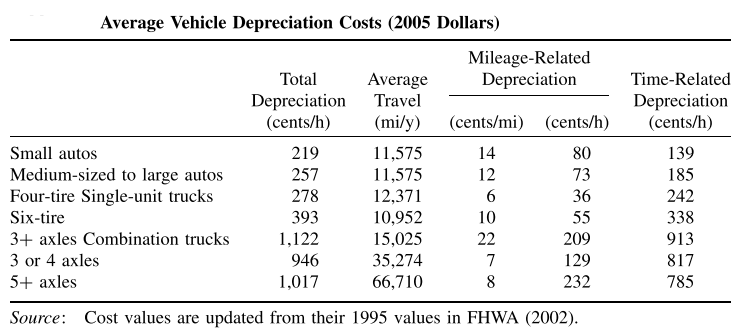
\includegraphics[scale=0.65]{gfx/fig63.png}
\end{center}
The values presented in the above table are average values. Depreciation rates actually vary by factors such as grade, curves, surface condition, and speed. An improvement in the transportation facility can produce a smoother pavement and improved driving conditions (through reduced stop-and-go situations). Also, all other factors remaining the same, increased speed can lead to reduced depreciation rates, as illustrated in the figure below, for straight constant-speed sections (FHWA, 2002).
\begin{center}
	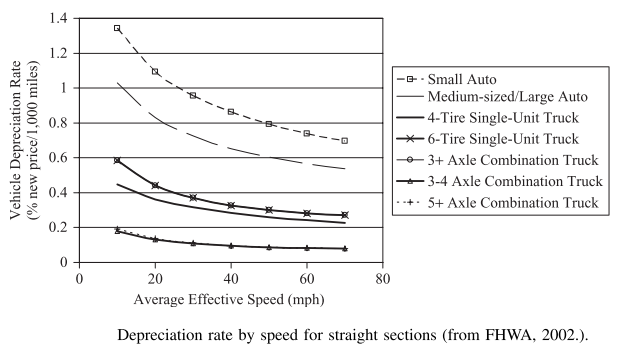
\includegraphics[scale=0.65]{gfx/fig64.png}
\end{center}
%%%%%
\section{Factors That Affect Vehicle Operating Cost}
For all modes of transportation, vehicle operating costs are affected by factors such as vehicle–operator characteristics, economic factors, condition and other characteristics of the fixed transportation facility, and policy–institutional factors. Although we focus on highway transportation in this section, the principles and concepts can be adapted to other transportation modes. The figure below shows the categories of highway VOC factors.
\begin{center}
	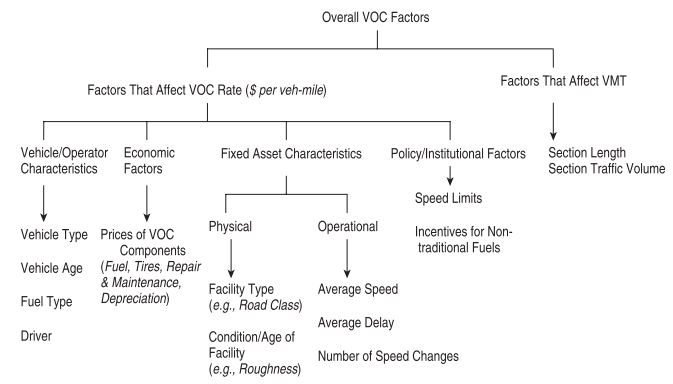
\includegraphics[scale=0.65]{gfx/fig65.png}
\end{center}
%%
\subsection{Vehicle Type}
Vehicle operating costs are influenced by size, class, and other vehicle characteristics. Trucks and buses generally have higher operating costs than automobiles, as they consume more fuel and oil and have higher prices for their vehicle parts. Even for a given vehicle type, there could be changes in VOC over time due to improved vehicle technology and fuel efficiency. If the analyst seeks to carry out long-term VOC impact evaluation, future levels of fuel efficiency could be extrapolated from past trends and duly factored in the VOC computation process.\\\\
In some cases, analysts may seek the operating costs associated with bicycling and walking to facilitate a more comprehensive comparison of transportation alternatives that include these modes. A standard bicycle with basic accessories can cost \$100 to \$500 with annualized maintenance costs of \$20 to \$40 for tire replacement, tire pumping, and security; for walking, the main consumable is that of footwear, which typically lasts 500 to 5000 miles of walking distance (VTPI, 2004). The human energy use associated with walking and cycling may be considered a benefit rather than a cost, particularly if traveling using these transportation modes substitute for other exercise activities.
%%
\subsection{Fuel Type}
The uncertainties in supply and increasing costs of fossil fuels coupled with their adverse environmental effects have led to growing use of alternative energy sources for transportation. In evaluating the impacts of transportation improvements, therefore, analysts need to account for the increasing percentage of alternative-fuel vehicles in the traffic stream. At the current time, electric and hybrid vehicles have relatively high purchase costs (150 to 200\% of the price of a comparable gasoline car). Electric cars require new battery sets every 20,000 to 30,000 miles costing \$2000 to \$3000 (averaging 6 to 15 cents per vehicle-mile), and consume 0.25 to 0.5 kWh per mile, so energy costs average 2 to 5 cents per kWh based on typical residential energy rates (USDOE, 2005a). The maintenance costs, including battery replacements, are significantly higher for electric cars (over four fold) compared to hybrid or conventional cars (VTPI, 2005). Even with traditional fuels, there are differences in cost across fuel types: in 2005, the average price of diesel was approximately 10\% higher than that of regular leaded gasoline. Also, there are price differences across the three standard grades of gasoline.
%%
\subsection{Longitudinal Grade} 
Uphill movements impose additional loads on vehicle engines and therefore require greater consumption of energy compared to downhill or level movements. For downhill trips, fuel consumption is lower than for uphill or level trips, but increased brake applications may lead to increased wear and tear of brake linings and therefore to increased cost of the brake maintenance component of VOC. The figure below illustrates the general relationships between grade and VOC at various speeds for medium-sized automobile. Generally, overall VOC is lowest for sections with gentle downward slopes (0 to -4\%).
\begin{center}
	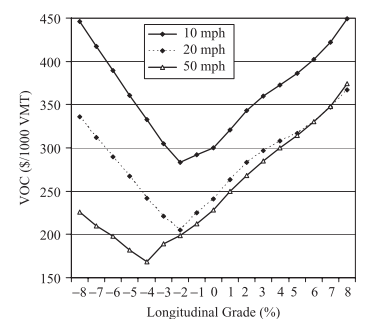
\includegraphics[scale=0.7]{gfx/fig66.png}
\end{center}
\textbf{\textit{Numerical Example:}}\\\\
A 2.15-mile section of State Road 25 on rolling terrain received major improvements in vertical alignment. The average grade of the section was reduced from 3.2\% to 2.5\%. Traffic volume and composition, and speed were the same after the improvement. Assume that the traffic stream has a 50:50 directional split and is composed primarily of medium-sized automobiles, and the traffic volume is 43,340 vpd (vehicles per day). In both cases, the average speed is 50 mph. What is the first year user benefit in terms of VOC?\\
\textit{Solution:}\\\\
Section Length (L) = 2.15 mile\\
Average Daily Traffic (ADT) = 43340 vpd\\
Average speed of the vehicle (v) = 50 mph\\\\
Before Improvement:\\
uphill: VOC at +3.2\% grade ($ {VOC}_1 $) = \$ 275/1000 VMT (using graph for medium-sized automobile)\\
downhill: VOC at -3.2\% grade ($ {VOC}_2 $) = \$ 190/1000 VMT (using graph for medium-sized automobile)\\
Average VOC before improvement ($ U_1 $) = $ \frac{275 + 190}{2} $ = \$232.5/1000 VMT\\
Vehicle Miles Travelled per year ($ {VMT}_1 $) = $ L \times ADT \times 360 = 2.15 \times 43340 \times 360 $ = 34011035 vehicle miles per year\\\\
After Improvement:\\
uphill: VOC at +2.5\% grade ($ {VOC}^{'}_1 $) = \$ 260/1000 VMT (using graph for medium-sized automobile)\\
downhill: VOC at -2.5\% grade ($ {VOC}^{'}_2 $) = \$ 200/1000 VMT (using graph for medium-sized automobile)\\
Average VOC after improvement ($ U_2 $) = $ \frac{260 + 200}{2} $ = \$230/1000 VMT\\
$ \because $ the traffic volume remains unchanged after improvement in longitudinal grade,\\
$ {VMT}_2 = {VMT}_1 $\\\\
Now,\\
Change in unit costs ($ U_1 - U_2 $) = 232.5 - 230 = 2.5/1000 VMT = 0.0025 VMT\\\\
$ \therefore $ First year user benefits = $ 0.5 \times (U_1 - U_2) \times ({VMT}_1 + {VMT}_2) $\\ = $ 0.5 \times 0.0025 \times 2 \times 34011065$ = \$ 85028
%%
\subsection{Vehicle Speed}
Vehicle operating speed is the dominant factor in determining VOC (Bennett, 1991; Thoresen and Roper, 1996; Bennett and Greenwood, 2001; FHWA, 2002). Transportation improvements influence travel speeds and therefore can profoundly affect VOC. For some vehicles, fuel consumption decreases with increasing speed to a certain point, after which there is little significant change (or sometimes, an increase) in fuel consumption with increasing speed. Factors that affect operating speeds, and subsequently influence fuel VOC, are speed limits (set by policy) and traffic conditions (which vary by the time of day—peak vs. nonpeak). In this section we discuss the impact of speed on shipping inventory costs and present some VOC models based on speed and other factors.
\subsubsection{a) Inventory Shipping}
Inventory cost is affected by vehicle speed and is calculated as follows:
\begin{equation}
	U_{IC} = 100 \times \frac{r}{365 \times 24} \times \frac{1}{S} \times P
\end{equation}
where $ U_{IC} $ is the user inventory cost in cents per vehicle mile, $ r $ the annual interest rate, $ P $ the cargo value in dollars, and $ S $ the vehicle speed in miles per hour.\\\\
\textbf{\textit{Numerical Example:}}\\
Due to a new speed limit policy, the average truck operating speed on a certain interstate freeway increased from 56.5 mph to 61.2 mph. Find the decrease in shipping inventory costs per year for trucks that comprise 22\% of the overall traffic stream of 82,500 vehicles per day (vpd). Each truck hauls an average of \$1.5 million worth of goods daily. Assume an 8\% interest rate.\\
\textit{Solution:}\\\\
The daily changes in inventory costs per truck due to the change in travel speed, $ \Delta U_{IC} $, can be estimated as follows:\\
$ \Delta U_{IC} = 100 \times \frac{r}{365 \times 24} \times \left( \frac{1}{S_0} - \frac{1}{S_1} \right) \times P$\\
$ 100 \times \frac{0.08}{365 \times 24} \times \left( \frac{1}{56.5} - \frac{1}{61.2} \right) \times 1500000 $\\
$ \therefore \Delta U_{IC} = 1.9178 $ cents/vehicle-mike\\\\
Then,\\
Number of trucks per year = (0.22)(82,500)(365) = 6,624,750\\
$ \therefore $ total reduction in inventory costs for all trucks per year = (1.9178/100)(6,624,750) = \$127,050 per mile
%%
\subsubsection{b) VOC Models and Look-up Table Based on Speed and Vehicle Class}
Hepburn (1994) developed a VOC model for urban roadways that considers the sum of four VOC components (tires, vehicle depreciation, maintenance, and fuel) as a function of two VOC factors: speed and vehicle class. The model is particularly useful for evaluating VOC impacts of transportation interventions that mostly yield a change in average operating speeds or policies that cause a shift in vehicle class distribution. The Hepburn function is as follows:\\\\
For “low” average travel: speeds ($ < $ 50 mph)
\begin{equation}
	VOC = C + \frac{D}{S}
\end{equation}
For “high” average travel: speeds ($ > $ 50 mph)
\begin{equation}
	VOC = a_0 - a_1 \times S + a_2 \times S^2
\end{equation}
where VOC is in cents/mile, $ S $ is speed (mph) and $ C $, $ D $, $ a_0 $, $ a_1 $,and $ a_2 $ are coefficients that are functions of vehicle class. The coefficient values are given in the table below:
\begin{center}
	\begin{tabular}{c c c c c c}
		Vehicle Type & $ C $ & $ D $ & $ a_0 $ & $ a_1 $ & $ a_2 $\\
		\hline
		small automobile & 24.8 & 45.5 & 27.2 & 0.035 & 0.00021\\
		medium-sized automobile & 28.5 & 95.3 & 33.5 & 0.058 & 0.00029\\
		large automobile & 29.8 & 163.4 & 38.1 & 0.093 & 0.00033
	\end{tabular}
\end{center}
The Hepburn model assumes that depreciation depends
entirely on vehicle use and that the depreciation rate is constant throughout vehicle life. Furthermore, the model is for tangent, level, and urban road sections with pavement roughness assumed to remain constant over time, and all VOC component costs assumed to vary with distance, with the exception of fuel cost, which varies with speed. It does not explicitly consider the consumption rates and prices of individual VOC components for each vehicle class but is nevertheless useful for quick estimation of VOC.\\\\
\textbf{\textit{Numerical Example:}}\\
A straight and level urban arterial has an average operating speed of 35 mph. What is the unit VOC of medium-sized automobiles that use this highway?\\
\textit{Solution:}\\\\
Knowing the values of C and D from Table:\\\\
$ VOC = C + \frac{D}{S} = 28.5 + \frac{95.3}{35} $ = 31.22 cents/vehicle-mile
\subsubsection{c) VOC model based on speed, grade, and vehicle class}
Zaniewski (1982) provided a VOC model as a function of speed, grade, and vehicle class. Table 7.4 presents the VOCs for medium-sized autos, with updated cost values. If the project section consists of several segments with different grades or VMTs, the unit VOC (dollars/vehicle-mile) is estimated separately for each segment. It should be noted, however, that the vehicles at the time of the Zaniewski study (ca. 1980) had 17\% lower fuel efficiency than vehicles in 1997 (FHWA, 2002), and even lower compared to vehicles in 2005. As such, Table given below should be used after stating the necessary assumptions regarding fuel efficiency, or after making due adjustments for fuel efficiency changes over the years.
\begin{center}
	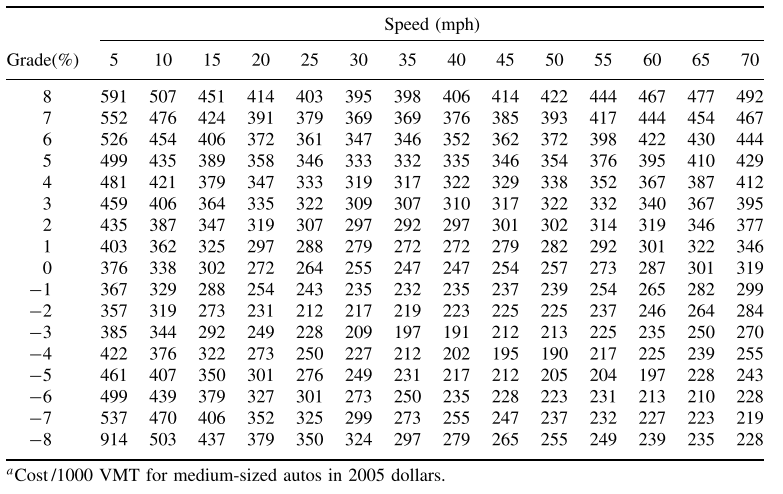
\includegraphics[scale=0.6]{gfx/fig67.png}
\end{center}
%
\textbf{\textit{Numerical Example:}}\\
A highway section consists of two segments A and B that have the characteristics listed in table below. Determine the total vehicle operating costs for each segment. Assume that all vehicles are medium sized automobiles, and assume further that the values in the table reflect current fuel consumption rates.
\begin{center}
	\begin{tabular}{p{3.5 cm} p{3.5 cm} p{3.5 cm}}
		\hline
		 & Segment A & Segment B\\
		 \hline
		 Traffic volume (ADT) & 5320 & 8580\\
		 Average grade (\%) & +4 & +1.5\\
		 Speed (mph) & 30 & 50\\
		 length (miles) & 5.7 & 2.6\\
		 Directional Split & 68\% (upward slope); 32\% (downward slope) & 45\% (upward slope); 55\% (downward slope)\\
		 \hline
	\end{tabular}
\end{center}
\textit{Solution:}\\
Segment A:\\\\
Total Unit VOC = Unit VOC for uphill + unit VOC for downhill\\
\hspace*{2cm} = $ unitVOC_{vehicle speed, grade, vehicle class} $ $ \times $ uphill directional split + $ unitVOC_{vehicle speed, grade, vehicle class} $ $ \times $ downhill directional split\\
\hspace*{2cm} = 319 $ \times $ 0.68 + 227 $ \times $ 0.32 = \$289.56/1000 VMT\\\\
VMT = section length $ times $ ADT = 5.7 $ \times $ 5320 = 30325 vehicle-miles per day\\\\
Overall VOC = Total unit VOC $ \times$ VMT = $ \frac{289.56}{1000} \times 30325 $ = \$8781 per day\\\\
Segment B:\\\\
Total Unit VOC = Unit VOC for uphill + unit VOC for downhill\\
\hspace*{2cm} = uphill grade $ \times $ uphill directional split + downhill grade $ \times $ downhill directional split\\
\hspace*{2cm} = 292 $ \times $ 0.45 + 232 $ \times $ 0.55 = \$259/1000 VMT\\\\
VMT = section length $ times $ ADT = 2.6 $ \times $ 8580 = 22308 vehicle-miles per day\\\\
Overall VOC = Total unit VOC $ \times$ VMT = $ \frac{259}{1000} \times 22308 $ = \$5778 per day
\subsubsection{d) VOC Models Based on Speed, Gradient, Curvature, and Pavement Condition}
Some VOC models, such as the World Bank’s HDM (Bennett and Greenwood, 2001) and the HERS model (FHWA, 2002), estimate the unit cost of each VOC component as a function of speed, grade, and pavement condition. This is done for basic sections (straight sections with constant speed), and then excess vehicle operating costs due to speed changes and curvature are calculated. The excess VOC is added to the basic costs to yield the overall VOC for the section.
%%
\subsection{Delay}
Nodes and links in the networks of various transportation modes may often experience delay, which translates into higher vehicle operating costs. In evaluating transportation improvements at such facilities, VOC costs, particularly for fuel and inventory, can be expressed as a function of time delay. On highway links, for instance, delay can involve decelerating to a stop, idling, and accelerating from a stopped position. Such stop-and-go traffic leads to additional strain on a vehicle, which is translated into higher use of fuel and oil. All three phases involve fuel consumption rates that generally exceed that of constant-speed travel. The primary share of overall delay costs is attributed to acceleration of vehicles after being slowed or stopped rather than fuel consumed in decelerating or idling during delay periods (AASHTO, 2003). The impact of travel delay on VOC (fuel and inventory shipping cost components) can be estimated using a methodology provided by AASHTO (2003). In the methodology, the analyst estimates the delay with and without improvement using field measurements (applicable only to the existing situation), simulation, or analytical travel delay models. Using the estimated change in delay, fuel consumption rates per minute of delay and fuel price, the total cost of delay can be calculated.
\begin{center}
	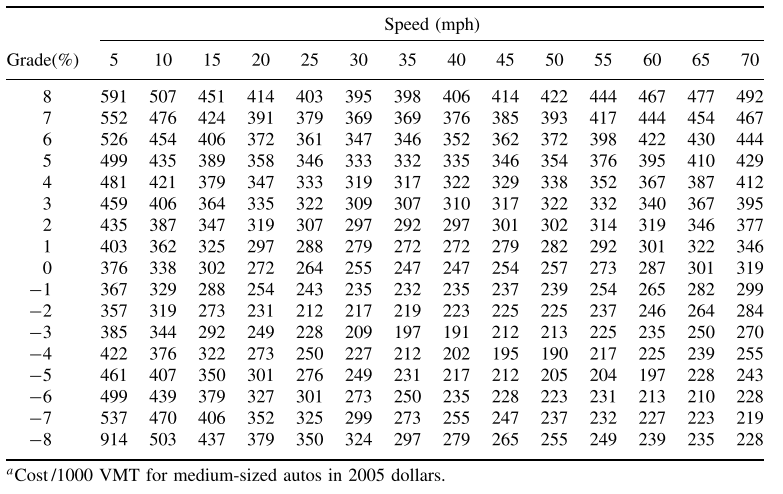
\includegraphics[scale=0.57]{gfx/fig67.png}
\end{center}
%
\subsubsection{a) Change in Fuel Costs due to Delay Change}
For a given vehicle class, the change in fuel costs due to a change in travel delay is found as follows (AASHTO, 2003):
\begin{equation}
	change \: in \: fuel \: VOC = g \times (D_0 - D_1 \times p)
\end{equation}
where: $ g $ is the fuel consumption in gallons per minute of delay (from the above table), $ D_0 - D_1 $ = change in delay (minutes) due to transportation improvement, and $ p $ is the price of the fuel. The parameters $ g $ and $ p $ are specific to vehicle class.\\\\
\textbf{\textit{Example:}}\\
Modernization and optimization of the traffic signal system at a busy urban arterial yielded, on average, a 9-minute reduction in delay per trip for users of the arterial. The traffic volume is 4300 vph and is composed of 25\% small autos, 30\% large autos, 25\% SUVs, 10\% two-axle single-unit trucks, 5\% three axle single-unit trucks, and 5\% multiple-unit trucks. After improvement, average free-flow speed increases from 45 mph to 50 mph, and traffic volume and composition remain unchanged. Determine the reduction in fuel costs during peak hours due to the decrease in delay. Assume that fuel cost is \$2.20 per gallon. Use the fuel consumption rates provided in the table above, and assume simple averages across vehicle classes.\\\\
\textit{Solution}:\\
The traffic volume for each vehicle class is determined by multiplying the percentage composition by the total traffic volume. Using the table above, the fuel consumption rates are determined, and the change in fuel consumption cost is presented the table below.
\begin{center}
	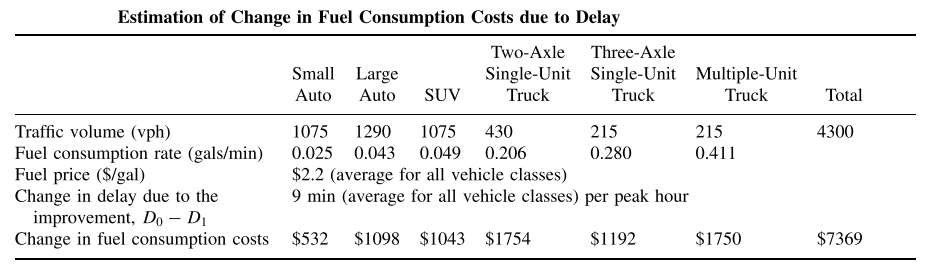
\includegraphics[scale= 0.55]{gfx/fig68.png}
\end{center}
Therefore, the total reduction in fuel costs during the peak hours due to the decrease in delay is \$7,369/hr.
%
\subsubsection{b) Change in Shipping Inventory Costs due to Delay}
AASHTO (2003) provides a methodology for estimating the impact of time delay on shipping operating costs, as follows: The change in inventory cost per shipping vehicle due to a change in delay is given by $ \Delta I(D) I(D) \times \Delta D $, where $ \Delta D $ is the change in delay (minutes) and inventory costs (cents per vehicle-minute) is given by,
\begin{equation}
	I(D) = 100 \times \frac{r}{365 \times 24 \times 60} \times P
\end{equation}
where $ r $ is the interest rate (per annum) and $ P $ is the dollar value of the cargo being transported by the shipping vehicle.\\\\
In some cases, the analyst is provided with an estimate of the expected change in delay, but in other cases, change in delay will need to be estimated (by calculating the delay before and after the improvement). Delay can be estimated on the basis of prevailing traffic conditions and road inventory.\\\\
Numerical Example:\\
A freeway was constructed in 2005 to bypass a city center. This improvement led to a 10-minute reduction in travel delay per trip for shippers who transport goods across the city. If the average value of cargo is \$265,000 per truck and the interest rate is 6\%, determine (a) the shipping inventory costs per vehicle before the construction, (b) the reduction in shipping inventory costs due to the construction in 2005, and (c) the change in user benefits accrued to shippers in 2005 compared to pre-construction conditions. The pre-construction period daily truck traffic (ADTT) was 33,000, and the trip time was 1.5 hours. Assume a 5\% ADTT increase due to induced demand.\\
Solution:\\
a) Shipping inventory cost per truck\\
The unit inventory cost of the shipment before improvement can be calculated as follows:\\
$ I(D) = P \times [r/(365 \times 25 \times 60)] = 265000 \times [0.06/(365 \times 25 \times 60)] = \$0.03025/truck-minute $\\\\
The unit inventory cost after the improvement is the same as that before the improvement because there is no change in the total cargo value and the annual interest rate. Since the travel time reduces by 10 minutes after the improvement, the total inventory cost saved due to the improvement is\\
Change in unit inventory cost = $ \$0.03025/truck-minute \times 10 \: minutes $ = \$0.3025/truck\\\\
b) Reduction in Shipping Inventory Cost\\
The unit shipping inventory cost in dollars/truck-mile, U, can be calculated as follows:\\
Before Improvement:\\\\
$ U_{before} = \$0.03025/truck-minute \times (60/S_{before}) $ = \$1.815T/L per truck-mile\\\\
where $ S_{before} $ = average speed before improvement (mph) = $ L/T $, $ L $ = average truck trip length (miles) and $ T $ = average truck trip time (hours).\\\\
$ \therefore $ Total yearly inventory cost = (\$1.815T/L)(ADTT)(L)(365)\\\\
After Improvement:\\\\
$ U_{after} = \$0.03025/truck-minute \times (60/S_{after})$ = \$1.815[T - (10/60)]/L per truck-mile\\\\
Therefore, the reduction in total shipping inventory cost = Total yearly inventory cost before the improvement - Total yearly inventory cost after the improvement = 1.815 ADTT (365) [T- 1.05{T- (10/60)}] = 1.815 ADTT (365) [0.175 - 0.05T] = \$2,186,168 in the first year.\\\\
c) Change in user benefit (Change in consumer surplus)\\\\
The change in user benefits can be calculated based on the change in consumer surplus, which is given by the following formula:\\\\
User Benefits = $ \frac{1}{2} \times (U_{before} -U_{after}) \times (VMT_{before} + VMT_{after})$\\
\hspace*{2cm} = 0.5 ([(1.815 (10/60)/L)][2.05 ADTT (L)(365)] = = \$3,734,703.
%
\subsection{Speed Changes}
Vehicles travel at different speeds due to geometric and/or traffic conditions. It has been shown that the more frequent the speed change of a vehicle, the higher the associated operating cost, particularly its fuel component. When vehicles slow down or pick up speed, they experience additional strain that is translated into a higher use of fuel and oil. As such, highway projects that smoothen traffic flow by reducing the frequency and intensity of speed changes ultimately reduce the costs of vehicle operation.\\\\
An extreme case of speed change is stop–start conditions, which are usually typical of city driving. Barnes and Langworthy (2003) showed that for maintenance, repair, and depreciation, worsening stop–start conditions will increase costs of fuel consumption and to a smaller extent, the costs of maintenance, repair, and depreciation.
%
\subsection{Horizontal Curvature}
A vehicle negotiating a horizontal curve requires extra energy to counter centrifugal forces in order to stay in a radial rather than a tangential path. Furthermore, the side friction increases tire wear and tear, and the frequency and cost of maintenance and replacement. The VOC due to curves involves fuel, tire, and maintenance and repair, and is typically expressed as a function of the rate of consumption and unit prices of these VOC components, vehicle type, and average speed. In the HERS methodology, VOC for curve negotiation speed is estimated separately for sections with low speeds ($ <55 $ mph) and those with high speeds ($ > $55 mph).
%
\subsection{Road Surface Condition}
To some extent, pavement roughness, often measured in terms of the present serviceability index (PSI) or international roughness index (IRI), can affect the maintenance, tire, repair, and depreciation cost components of VOC. This is because the motion of vehicle tires on a rough pavement surface is associated with greater resistance to movement, which can lead to higher levels of fuel consumption compared to traveling at a similar speed on a smooth surface; and a bumpy ride, which leads to increased vibration and wear and tear of vehicle parts. Also, an indirect effect of poor pavement conditions is that road users may be forced to drive at lower speeds, leading to higher fuel consumption. Transportation projects such as resurfacing that improve pavement surfaces can therefore lead to reductions in VOCs.\\\\
Zaniewski (1982) suggested that there can be significant impacts of pavement roughness on nonfuel vehicle operating cost components, particularly for rough pavements. Most other research on the relationship between pavement condition and VOC has been conducted outside the United States by the World Bank and other international agencies. Examples include a New Zealand study (Opus Central Laboratories, 1999) which suggests that at superior levels of pavement condition (low roughness), increments in condition have relatively little incremental effect on vehicle operating cost (Figure 7.4), and that additional costs of vehicle operation start to accrue only when the IRI exceeds approximately 100 in/mi (3.33 m/km). For paved roads in poor condition and for gravel roads, changes in road surface condition can lead to significant reductions in VOC. Barnes and Langworthy (2003) reported on a previous study that suggested that a unit increase in IRI (in m/km) can generally lead to an increase of \$200 (1.67 cents/vehicle-mile, assuming 12,000 annual mileage) in vehicle maintenance and repair costs alone. Also, Barnes and Langworthy (2003) developed adjustment factors for all VOC components combined, as a function of pavement condition (in the figure below). They assumed a baseline PSI of 3.5 or better (an IRI of about 85 in/mi or 1.35 m/km), at which further increases in pavement condition would have no impact on operating costs, and then adjusted for three levels of rougher pavement as shown in the figure. The figure can be used to estimate the VOC corresponding to a given pavement condition. For the depreciation component, there seem to be relatively few studies that have explicitly shown a relationship with pavement roughness. However, it seems obvious that in the long term, a vehicle which is operated on a rough pavement surface is likely to lose its value faster than one that is operated on a smooth-surfaced pavement.
\begin{center}
	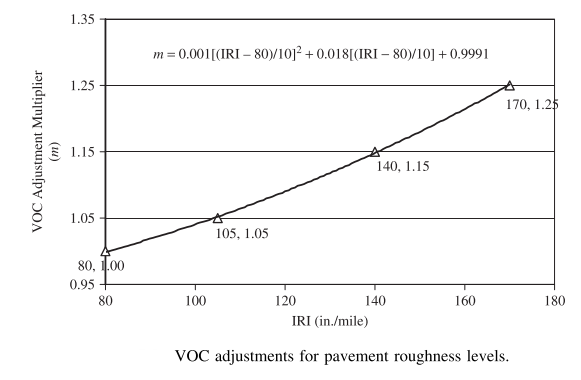
\includegraphics[scale=0.6]{gfx/fig69.png}
\end{center}
\textbf{\textit{Numerical Example:}}\\
A warranty HMA resurfacing project on Interstate 599 yielded a performance jump of 40 IRI (in/mi). If the base vehicle operating cost is \$143 per 1000 vehicle-miles, (a) determine the change in unit VOC due to resurfacing. Use the Barnes and Langworthy relationship. The IRI before improvement was 110 in/mi. (b) If the traffic volume is 67,500 vpd and the section is 6.5 miles in length, determine the overall change in VOC.\\
\textit{Solution:}\\
a) Before Improvement:\\
IRI = 110 in/mi, and the VOC adjustment multiplier is given by\\\\
m = $ 0.001 \times \left( \frac{110 - 80}{10} \right)^2 + 0.018 \times \frac{110 - 80}{10} + 0.9991 = 1.06$ \\\\
$ \therefore VOC $ = (1.06)(143) = \$151.58/1000 VMT\\\\
b) After Improvement:\\
IRI = 110 - 40 = 70 in/mi, m = 1.00 since 70 is less than 80, and therefore VOC = \$143/1000 VMT. Change
in unit VOC = 151.58 - 143 = \$8.58/1000 VMT.\\\\
$ \therefore $ Overall Change in VOC = (\$8.58)(67,500)(365) (6.5)/1000 = \$1.374 million.
%
\subsection{Other VOC Factors}
Other factors that can influence the cost of vehicle
operation include driver behavior, condition of vehicle, vehicle weight, prices of vehicle maintenance (reflected in costs of labor, vehicle consumables, and spare parts), and weather severity. Operating costs for transit vehicles (such as buses and trolleys) are also affected by other factors, such as transit schedules (which typically depend on passenger demand) and vandalism.
%%
\section{Procedure for Assesing VOC Impacts}
The framework for assessing VOC impacts of transportation interventions revolves around three tasks:
\begin{enumerate}
	\item Estimating the unit VOC rates (i.e., dollars/vehiclemile) with and without intervention
	\item Estimating the amounts of travel (VMT) with and without the intervention
	\item Calculating the user VOC benefits of intervention
\end{enumerate}